% Options for packages loaded elsewhere
\PassOptionsToPackage{unicode}{hyperref}
\PassOptionsToPackage{hyphens}{url}
\PassOptionsToPackage{dvipsnames,svgnames,x11names}{xcolor}
%
\documentclass[
  letterpaper,
  DIV=11,
  numbers=noendperiod]{scrartcl}

\usepackage{amsmath,amssymb}
\usepackage{iftex}
\ifPDFTeX
  \usepackage[T1]{fontenc}
  \usepackage[utf8]{inputenc}
  \usepackage{textcomp} % provide euro and other symbols
\else % if luatex or xetex
  \usepackage{unicode-math}
  \defaultfontfeatures{Scale=MatchLowercase}
  \defaultfontfeatures[\rmfamily]{Ligatures=TeX,Scale=1}
\fi
\usepackage{lmodern}
\ifPDFTeX\else  
    % xetex/luatex font selection
\fi
% Use upquote if available, for straight quotes in verbatim environments
\IfFileExists{upquote.sty}{\usepackage{upquote}}{}
\IfFileExists{microtype.sty}{% use microtype if available
  \usepackage[]{microtype}
  \UseMicrotypeSet[protrusion]{basicmath} % disable protrusion for tt fonts
}{}
\makeatletter
\@ifundefined{KOMAClassName}{% if non-KOMA class
  \IfFileExists{parskip.sty}{%
    \usepackage{parskip}
  }{% else
    \setlength{\parindent}{0pt}
    \setlength{\parskip}{6pt plus 2pt minus 1pt}}
}{% if KOMA class
  \KOMAoptions{parskip=half}}
\makeatother
\usepackage{xcolor}
\setlength{\emergencystretch}{3em} % prevent overfull lines
\setcounter{secnumdepth}{-\maxdimen} % remove section numbering
% Make \paragraph and \subparagraph free-standing
\ifx\paragraph\undefined\else
  \let\oldparagraph\paragraph
  \renewcommand{\paragraph}[1]{\oldparagraph{#1}\mbox{}}
\fi
\ifx\subparagraph\undefined\else
  \let\oldsubparagraph\subparagraph
  \renewcommand{\subparagraph}[1]{\oldsubparagraph{#1}\mbox{}}
\fi

\usepackage{color}
\usepackage{fancyvrb}
\newcommand{\VerbBar}{|}
\newcommand{\VERB}{\Verb[commandchars=\\\{\}]}
\DefineVerbatimEnvironment{Highlighting}{Verbatim}{commandchars=\\\{\}}
% Add ',fontsize=\small' for more characters per line
\usepackage{framed}
\definecolor{shadecolor}{RGB}{241,243,245}
\newenvironment{Shaded}{\begin{snugshade}}{\end{snugshade}}
\newcommand{\AlertTok}[1]{\textcolor[rgb]{0.68,0.00,0.00}{#1}}
\newcommand{\AnnotationTok}[1]{\textcolor[rgb]{0.37,0.37,0.37}{#1}}
\newcommand{\AttributeTok}[1]{\textcolor[rgb]{0.40,0.45,0.13}{#1}}
\newcommand{\BaseNTok}[1]{\textcolor[rgb]{0.68,0.00,0.00}{#1}}
\newcommand{\BuiltInTok}[1]{\textcolor[rgb]{0.00,0.23,0.31}{#1}}
\newcommand{\CharTok}[1]{\textcolor[rgb]{0.13,0.47,0.30}{#1}}
\newcommand{\CommentTok}[1]{\textcolor[rgb]{0.37,0.37,0.37}{#1}}
\newcommand{\CommentVarTok}[1]{\textcolor[rgb]{0.37,0.37,0.37}{\textit{#1}}}
\newcommand{\ConstantTok}[1]{\textcolor[rgb]{0.56,0.35,0.01}{#1}}
\newcommand{\ControlFlowTok}[1]{\textcolor[rgb]{0.00,0.23,0.31}{#1}}
\newcommand{\DataTypeTok}[1]{\textcolor[rgb]{0.68,0.00,0.00}{#1}}
\newcommand{\DecValTok}[1]{\textcolor[rgb]{0.68,0.00,0.00}{#1}}
\newcommand{\DocumentationTok}[1]{\textcolor[rgb]{0.37,0.37,0.37}{\textit{#1}}}
\newcommand{\ErrorTok}[1]{\textcolor[rgb]{0.68,0.00,0.00}{#1}}
\newcommand{\ExtensionTok}[1]{\textcolor[rgb]{0.00,0.23,0.31}{#1}}
\newcommand{\FloatTok}[1]{\textcolor[rgb]{0.68,0.00,0.00}{#1}}
\newcommand{\FunctionTok}[1]{\textcolor[rgb]{0.28,0.35,0.67}{#1}}
\newcommand{\ImportTok}[1]{\textcolor[rgb]{0.00,0.46,0.62}{#1}}
\newcommand{\InformationTok}[1]{\textcolor[rgb]{0.37,0.37,0.37}{#1}}
\newcommand{\KeywordTok}[1]{\textcolor[rgb]{0.00,0.23,0.31}{#1}}
\newcommand{\NormalTok}[1]{\textcolor[rgb]{0.00,0.23,0.31}{#1}}
\newcommand{\OperatorTok}[1]{\textcolor[rgb]{0.37,0.37,0.37}{#1}}
\newcommand{\OtherTok}[1]{\textcolor[rgb]{0.00,0.23,0.31}{#1}}
\newcommand{\PreprocessorTok}[1]{\textcolor[rgb]{0.68,0.00,0.00}{#1}}
\newcommand{\RegionMarkerTok}[1]{\textcolor[rgb]{0.00,0.23,0.31}{#1}}
\newcommand{\SpecialCharTok}[1]{\textcolor[rgb]{0.37,0.37,0.37}{#1}}
\newcommand{\SpecialStringTok}[1]{\textcolor[rgb]{0.13,0.47,0.30}{#1}}
\newcommand{\StringTok}[1]{\textcolor[rgb]{0.13,0.47,0.30}{#1}}
\newcommand{\VariableTok}[1]{\textcolor[rgb]{0.07,0.07,0.07}{#1}}
\newcommand{\VerbatimStringTok}[1]{\textcolor[rgb]{0.13,0.47,0.30}{#1}}
\newcommand{\WarningTok}[1]{\textcolor[rgb]{0.37,0.37,0.37}{\textit{#1}}}

\providecommand{\tightlist}{%
  \setlength{\itemsep}{0pt}\setlength{\parskip}{0pt}}\usepackage{longtable,booktabs,array}
\usepackage{calc} % for calculating minipage widths
% Correct order of tables after \paragraph or \subparagraph
\usepackage{etoolbox}
\makeatletter
\patchcmd\longtable{\par}{\if@noskipsec\mbox{}\fi\par}{}{}
\makeatother
% Allow footnotes in longtable head/foot
\IfFileExists{footnotehyper.sty}{\usepackage{footnotehyper}}{\usepackage{footnote}}
\makesavenoteenv{longtable}
\usepackage{graphicx}
\makeatletter
\def\maxwidth{\ifdim\Gin@nat@width>\linewidth\linewidth\else\Gin@nat@width\fi}
\def\maxheight{\ifdim\Gin@nat@height>\textheight\textheight\else\Gin@nat@height\fi}
\makeatother
% Scale images if necessary, so that they will not overflow the page
% margins by default, and it is still possible to overwrite the defaults
% using explicit options in \includegraphics[width, height, ...]{}
\setkeys{Gin}{width=\maxwidth,height=\maxheight,keepaspectratio}
% Set default figure placement to htbp
\makeatletter
\def\fps@figure{htbp}
\makeatother

\KOMAoption{captions}{tableheading}
\makeatletter
\makeatother
\makeatletter
\makeatother
\makeatletter
\@ifpackageloaded{caption}{}{\usepackage{caption}}
\AtBeginDocument{%
\ifdefined\contentsname
  \renewcommand*\contentsname{Table of contents}
\else
  \newcommand\contentsname{Table of contents}
\fi
\ifdefined\listfigurename
  \renewcommand*\listfigurename{List of Figures}
\else
  \newcommand\listfigurename{List of Figures}
\fi
\ifdefined\listtablename
  \renewcommand*\listtablename{List of Tables}
\else
  \newcommand\listtablename{List of Tables}
\fi
\ifdefined\figurename
  \renewcommand*\figurename{Figure}
\else
  \newcommand\figurename{Figure}
\fi
\ifdefined\tablename
  \renewcommand*\tablename{Table}
\else
  \newcommand\tablename{Table}
\fi
}
\@ifpackageloaded{float}{}{\usepackage{float}}
\floatstyle{ruled}
\@ifundefined{c@chapter}{\newfloat{codelisting}{h}{lop}}{\newfloat{codelisting}{h}{lop}[chapter]}
\floatname{codelisting}{Listing}
\newcommand*\listoflistings{\listof{codelisting}{List of Listings}}
\makeatother
\makeatletter
\@ifpackageloaded{caption}{}{\usepackage{caption}}
\@ifpackageloaded{subcaption}{}{\usepackage{subcaption}}
\makeatother
\makeatletter
\@ifpackageloaded{tcolorbox}{}{\usepackage[skins,breakable]{tcolorbox}}
\makeatother
\makeatletter
\@ifundefined{shadecolor}{\definecolor{shadecolor}{rgb}{.97, .97, .97}}
\makeatother
\makeatletter
\makeatother
\makeatletter
\makeatother
\ifLuaTeX
  \usepackage{selnolig}  % disable illegal ligatures
\fi
\IfFileExists{bookmark.sty}{\usepackage{bookmark}}{\usepackage{hyperref}}
\IfFileExists{xurl.sty}{\usepackage{xurl}}{} % add URL line breaks if available
\urlstyle{same} % disable monospaced font for URLs
\hypersetup{
  pdftitle={Theoretical study Quarto -document},
  colorlinks=true,
  linkcolor={blue},
  filecolor={Maroon},
  citecolor={Blue},
  urlcolor={Blue},
  pdfcreator={LaTeX via pandoc}}

\title{Theoretical study Quarto -document}
\author{}
\date{2026-01-28}

\begin{document}
\maketitle
\ifdefined\Shaded\renewenvironment{Shaded}{\begin{tcolorbox}[boxrule=0pt, enhanced, borderline west={3pt}{0pt}{shadecolor}, interior hidden, breakable, sharp corners, frame hidden]}{\end{tcolorbox}}\fi

\hypertarget{to-do-4.2.}{%
\subsubsection{To do 4.2.}\label{to-do-4.2.}}

\begin{itemize}
\item
  Main consideration: Should measurement error be dropped from the s-LMI
  model and just call it autoregressive common factor model. This
  largely simplifies, and is justifiable in the sense that VAR(1) does
  not contain across time point measurement errors (innovations).
\item
  Add/integrate previous Rmd file of theoretical result as extension to
  this one.
\item
  Recheck delta t.
\item
  Check if subindex VAR(1) is necessary for Sigma.
\item
  Integrating Tom's notes (26.1 onwards)
\item
  Serially independent innovations force the
\item
  Many proofs are currently in scratch file, accessible from there.
\end{itemize}

\hypertarget{empirical-distinguishability}{%
\subsubsection{Empirical
distinguishability}\label{empirical-distinguishability}}

\begin{description}
\item[Common Factor theoretical model]
A latent variable \(\eta\) is a causal entity which creates observable
symptoms. Conditional independence of variables
\(P(X_i|\eta,X_j)=P(X_i|\eta):\:i\ne j\) given the common factor
\(\eta\) is the central proposition of the model. All changes in
symptoms are due to changes in \(\eta\). \(M_1\) will represent an
empirical (data-generating) model of the common factor theory.
\item[Mutualistic symptom-network theoretical model]
Symptoms have causal effects on each others. Symptoms can change by
themselves or change due to effects not within the symptom-network
itself. The symptom-network is all the symptoms. \(M_2\) will represent
an empirical (data-generating) model of the symptom-network theory.
\end{description}

The models need to be kept vague for now, as the key parts of both
differ in each scenario to be examined. Empirical distinguishability is
here defined up to the fourth order moment:

\begin{description}
\item[Empirical distinguishability]
\[\begin{aligned} E_{M_1}(X)-E_{M_2}(X)&=D_E\\\   \text{Cov} _{M_1}(X)-\text{Cov} _{M_2}(X)&=D_C  \\   \text{Skew} _{M_1}(X)-\text{Skew} _{M_2}(X)&=D_S\\   \text{Kurt} _{M_1}(X)-\text{Kurt} _{M_2}(X)&=D_S   \end{aligned}  \]
\end{description}

That is, after defining the models, data simulated from both of these
models should always be the same w.r.t. their expectation, covariance,
skewness and kurtosis. Our aim is to identify practical conditions,
where the distinguishability is highest - i.e., when the differences in
either expectation or covariance become largest. We do this in X
different scenarios. In all scenarios we define a respective common
factor theory model as well as a symptom-network mutualism model. We
then aim to analytically show the differences between the models, and
then through simulation quantify what types of practical difference we
might see. We'll be denoting symptoms as random matrix \(X\), of which
columns are the symptoms. We use two theoretical models:

The several scenarios relate to study designs, in which both models have
been used using real world empirical data. First, we examine changes
over time. Second, \ldots, X:th.

\hypertarget{change-across-time-strict-longitudinal-measurement-invariance-vs-var1-models}{%
\subsubsection{Change across time: Strict Longitudinal Measurement
Invariance vs VAR(1)
models}\label{change-across-time-strict-longitudinal-measurement-invariance-vs-var1-models}}

Regarding changes in symptoms across time, the most basic models that we
can use for common factor and symptom-network theory are the strict
longitudinal measurement invariance (s-LMI) referred to as and the
vector autoregressive model of order one (VAR(1)). Here we will
analytically approach differences between these models and then perform
simulations to quantify how well empirically the models differ when
generating from a mixture distribution. We will first inspect what type
of covariance structure VAR(1) imposes, and then similarly s-LMI.

Their difference is not always evident. See for example the figure
below, where data was generated from both models.

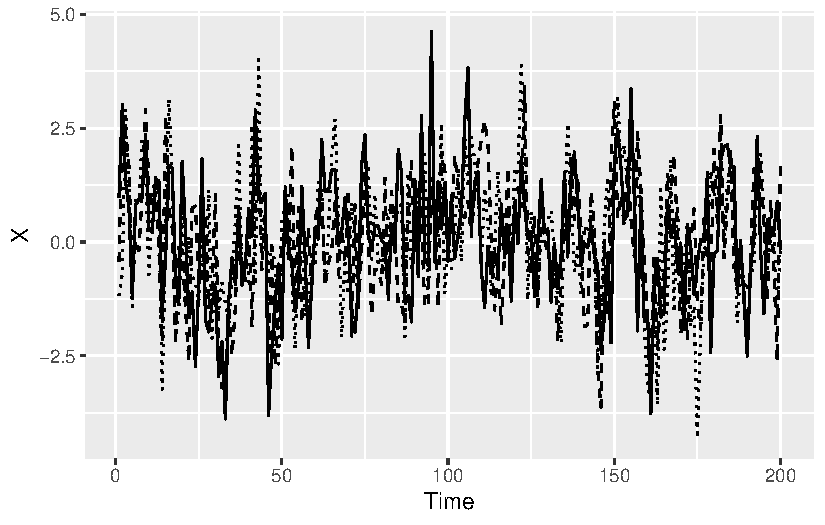
\includegraphics{TheoreticalStudy--1-_files/figure-pdf/unnamed-chunk-1-1.pdf}

The model was set up so that there is a true common factor \(\eta\)
causing three variables \(X\). The common factor had an autoregressive
coefficient (of order 1) of \(\sqrt{0.5}\approx0.7071\) to itself and
\(\psi_t \sim N(0, \sqrt{0.5})\) innovations (0.5 variance). Each of the
\(X_{i,t}\) also had their own measurement errors
\(\omega_{i,t}\sim N(0,\sqrt{0.5})\). \(X_t\) has a covariance matrix
approximately such that the diagonal elements are 2, and off-diagonal
elements are 1.

If simulating from another numerical example, this time a VAR(1)
process, we can observe a fairly similar looking pattern.

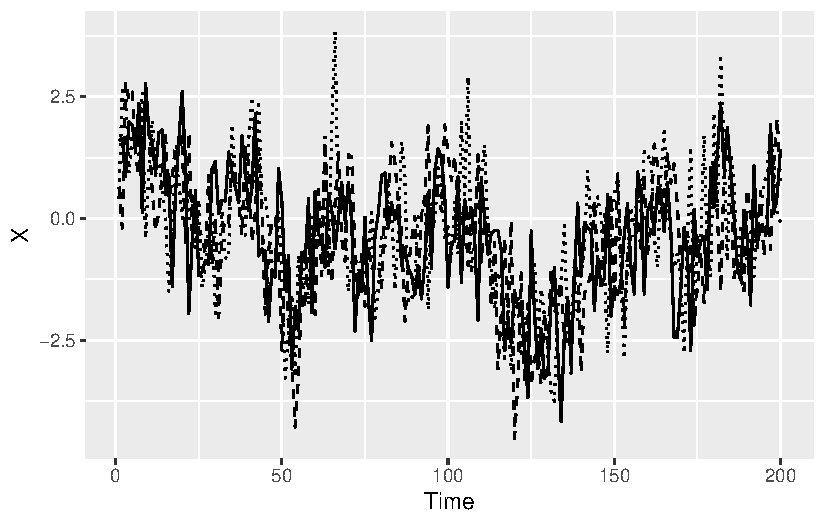
\includegraphics{TheoreticalStudy--1-_files/figure-pdf/unnamed-chunk-2-1.pdf}

The difference between the two example time series in \(D_C\) is

\begin{Shaded}
\begin{Highlighting}[]
\NormalTok{D\_C }\OtherTok{=}\NormalTok{ (}\FunctionTok{cov}\NormalTok{(X\_VAR) }\SpecialCharTok{{-}} \FunctionTok{cov}\NormalTok{(X\_CF))}
\FunctionTok{dimnames}\NormalTok{(D\_C) }\OtherTok{=} \FunctionTok{list}\NormalTok{(}\FunctionTok{paste}\NormalTok{(}\StringTok{"X"}\NormalTok{,}\DecValTok{1}\SpecialCharTok{:}\DecValTok{3}\NormalTok{,}\AttributeTok{sep =} \StringTok{""}\NormalTok{),}\FunctionTok{paste}\NormalTok{(}\StringTok{"X"}\NormalTok{,}\DecValTok{1}\SpecialCharTok{:}\DecValTok{3}\NormalTok{,}\AttributeTok{sep =} \StringTok{""}\NormalTok{))}
\FunctionTok{round}\NormalTok{(D\_C, }\DecValTok{2}\NormalTok{)}
\end{Highlighting}
\end{Shaded}

\begin{verbatim}
      X1    X2    X3
X1 -0.23  0.06 -0.14
X2  0.06 -0.09 -0.07
X3 -0.14 -0.07 -0.12
\end{verbatim}

\hypertarget{var1-covariance-structure}{%
\paragraph{VAR(1) covariance
structure}\label{var1-covariance-structure}}

Before the analysis, a brief theoretical consideration. We will assume
that the symptom-network represented as the VAR(1) model is a state.
This means that VAR(1) is stationary, and that there are no external
causes meaning that the innovations are uncorrelated - only symptoms can
correlate to each other. The VAR(1) model is defined in matrix format
for \(K\) symptoms as \(X_{t+1}=C+AX_{t}+\Gamma_t\), where \(\Gamma_t\)
is independent error column vector with \(E[\Gamma_t]=0\), \(C\) is a
constant assumed zero. Also assume centered \(X\), \(E[X_t]=0\), in our
case. Centering makes covariance calculations easier as the products of
expected values can be mostly ignored (they become 0). \(A\) is
\(K \times K\) (borrowing from CT-VAR terminology) `drift' matrix that
includes all lagged effects of \(K\times1\) column vectors \(X_t\) to
\(X_{t-1}\). \(A\) is independent of time. All matrices used are
real-valued.

First, the covariance matrix (assumed stationary over time) is

\[ \begin{align*} \text{Cov}(X_t) &= E[X_tX_t^T] \\ &= E[(AX_{t-1}+\Gamma_t)(AX_{t-1}+\Gamma_t)^T] \\ &= E[AX_{t-1}X_{t-1}^TA^T] + \underbrace{E[\Gamma_t \Gamma_t^T]}_{=: \Psi} \\ &= AE[X_{t-1}X_{t-1}^T]A^T + \Psi \\ &= \Sigma_t \end{align*} \]

The vectorized covariance matrix can be solved to equal\\
\[ \begin{align*} \text{vec}(\Sigma_{VAR(1)}) = (I-A \otimes A)^{-1} \text{vec}(\Psi) \end{align*} \]

Where vec is the vectorization operator and \(\otimes\) is the Kronecker
product. In the above the mixed Kronecker matrix vector product is used
to obtain the result. (Derivation is currently in a scratch file.)

Stationarity poses that \(\Sigma\) is not dependent of time. We will use
\(\Sigma_{VAR(1)}\) when we wish to be explicit about meaning the VAR(1)
imposed within time point covariance. \(\Gamma_t\) is a random
\(K\times1\) column vector of (serially) independent innovations at time
point \(t\), with \(E[\Gamma]=0\). \(\Psi\) is covariance of the
innovations within time point \(t\) - i.e., the contemporaneous
covariance. We assumed that the innovations are independent, as
described above, and so \(\Psi\) is diagonal. We use an arbitrary time
point \(t\) as the `first' measurement time point, so that time points
increase \({t, t+1,t+2,...,T}\), where \(T\) is the last measurement
time point. Here we focus on an across time point \(TK\times TK\)
covariance matrix. The \(TK\times TK\) covariance matrix will be denoted
as

\[ \begin{array}   
\\\Sigma_t&\Sigma_{t,t+1}&...&\Sigma_{t,T}
\\  \Sigma_{t+1,t}&\Sigma_{t+1}&...&\Sigma_{t+1,T}
\\ \vdots&\vdots&\ddots&\vdots   
\\ \Sigma_{T,t}^T&\Sigma_{T,t+1}^T&...&\Sigma_T \end{array} \]

Where the diagonal elements are within time points covariance matrices,
and off-diagonal elements are across time point covariance matrices. Let
\(^{(T)}\) denote the matrix raised to power of \(T\).

VAR(1) poses that observations at the time points \(X_t, X_{t-1}\) have
covariance \[
\begin{align*}
\text{Cov}(X_t,X_{t-1})&=
E[X_tX_{t-1}^T]-E[X_t]E[X_{t-1}]\\&=
E[(AX_{t-1}+\Gamma_t)X_{t-1}^T]\\&=
E[AX_{t-1}X_{t-1}^T]+E[\Gamma_tX_{t-1}^T]\\&=
A\Sigma_{t-1}+E[\Gamma_tX_{t-1}^T]
\end{align*}
\] Independent innovations means that
\(E[\Gamma_tX_{t-1}^T]=\text{Cov}(\Gamma_t,X_{t-1})=0\) leading to \[
\begin{align*}
\text{Cov}(X_t,X_{t-1})&= A\Sigma_{t-1}\\
\end{align*}
\]

This can be generalized to any two time points. The \(\Sigma_{t,T}\) for
VAR(1) is

\[ \Sigma_{t,T}=\text{Cov}(X_t, X_{t+\Delta t}) = A^{(\Delta t)}\Sigma_{VAR(1)} \]

(Above needs proof by induction for example.)

\hypertarget{s-lmi-covariance-structure-at-two-subsequent-time-points}{%
\paragraph{s-LMI covariance structure at two subsequent time
points}\label{s-lmi-covariance-structure-at-two-subsequent-time-points}}

We will use the s-LMI model to represent the common factor model for the
across time scenario. s-LMI is usually used with respect to measurement
development. However, it also makes a theoretical prediction as well.
s-LMI with 1 common factor decomposes \(\Sigma_{t}\) of \(K\) symptoms
into the following \[\Sigma_t=\Lambda\Lambda^T+\Omega\]where by
definition of s-LMI \(\Omega\) is diagonal and and \(\Lambda\) is a
\(K\times1\) column vector of factor loadings constant over time. We
also need the covariance of the common factor across time points. Let
\(\delta\) be the latent regression coefficient which links the common
factor to itself at a previous time point such that
\(\eta_{t+1}=\delta\eta_{t}+\psi_{t+1}\), where \(\psi_t\) is
independent random term mostly called measurement error with
\(E[\psi_t]=0\). Assuming standardized common factor such that
\(E[\eta_{t-1}]=0,\:Var(\eta_{t-1})=1\) covariance of the common factor
at two subsequent time points is

\[
\begin{align*} \text{Cov}(\eta_{t-1},\eta_t)= E[\eta_{t-1}\eta_t]-E[\eta_{t-1}]E[\eta_t]&=\\ E[\eta_{t-1}(\delta\eta_{t-1}+\psi_t)]&=\\ E[\delta\eta_{t-1}^2+\eta_{t-1}\psi_t]&=\\ \delta Var(\eta_{t-1})&= \delta \end{align*}
\]

Go straight to the general case !!!

Now lets look at the \(2K\times 2K\) covariance matrix from the
perspective of strict LMI. A s-LMI model imposes that \[
\text{Cov}((X_{t},X_{t-1}),(X_{t},X_{t-1}))= \begin{pmatrix}    \Lambda & 0
\\   0 & \Lambda \end{pmatrix}  \begin{pmatrix}   1 & \delta 
\\   \delta & \delta+Var(\psi_t) \end{pmatrix} \begin{pmatrix}    \Lambda^T & 0
\\   0 & \Lambda^T \end{pmatrix} + \begin{pmatrix}   \Omega_{t-1} & \Omega_{across} 
\\   \Omega_{across}^T & \Omega_t \end{pmatrix} 
\]

where

\[\begin{pmatrix}    \Lambda & 0\\   0 & \Lambda \end{pmatrix}\] is a
block matrix that sandwiches the \(2\times2\) covariance matrix of the
common factor at both time points.

\[
\begin{align*}&\begin{pmatrix}    \Lambda & 0\\   0 & \Lambda \end{pmatrix} \begin{pmatrix}   1 & \delta \\   \delta & \delta+Var(\psi_t) \end{pmatrix} \begin{pmatrix}    \Lambda^T & 0\\   0 & \Lambda^T \end{pmatrix}+ \begin{pmatrix}   \Omega_{t-1} & \Omega_{across} \\   \Omega_{across}^T & \Omega_t \end{pmatrix} =\\
&\begin{pmatrix}    \Lambda & 0\\   0 & \Lambda \end{pmatrix} \begin{pmatrix}    \Lambda^T & \delta\Lambda^T\\   \Lambda^T\delta & (\delta+Var(\psi_t)\Lambda^T \end{pmatrix} + 
\begin{pmatrix}   
\Omega_{t-1} & \Omega_{across} \\   
\Omega_{across}^T & \Omega_t \end{pmatrix}=\\
& \begin{pmatrix}    
\Lambda\Lambda^T + \Omega_{t-1}& \Lambda\Lambda^T\delta + \Omega_{across}\\   
\Lambda\Lambda^T\delta + \Omega_{across}^T & \Lambda\Lambda^T(\delta+Var(\psi_t)) + \Omega_t 
\end{pmatrix} 
\end{align*}
\] From the above we see that the strict LMI can only be compatible with
any process with stationary covariance, if
\(\delta+Var(\psi_t)=1\Rightarrow1-\delta=Var(\psi_t)\) (assuming
\(\Lambda\) is non-zero). (When fitting a s-LMI model this is allowed.)
We also see that s-LMI is compatible with non-stationary processes where
the covariance is proportional to \(\delta+Var(\psi_t)\) aligning with
previous theoretical analysis where covariance increased over time in a
LMI preserving model.

A brief note on notation: We'll be using simply \(\Omega\) for the s-LMI
residual covariance, since residual covariance is assumed invariant over
time \(\Omega_{t-1}=\Omega_{t}=\Omega_{t+1}=…=\Omega\) .

Using the above auxiliary results we can move to analyse the null
hypothesis (hypotheses) of no difference between VAR(1) and s-LMI.

\begin{description}
\item[Working null hypothesis (1)]
If covariance at some (measurement) time point is perfectly explained by
a common factor model with non-zero factor loadings \(\Lambda\), and if
the data generation is from a stationary VAR(1) model, then s-LMI model
fits perfectly.
\end{description}

Considering only the subset of VAR(1) processes which create a
covariance matrix that can be perfectly explained by a common factor
model is done because we're interested in how (if at all) VAR(1) can
deviate from s-LMI in terms of produced data. Understandably, if any
VAR(1) model creates covariance structure incompatible with s-LMI model
at some time point (i.e., a covariance matrix non-compatible with a
common factor model), then deviation must occur (although the extent to
which this occurs is not clear at this point).

If the VAR(1) generated \(2K\times2K\) matrix cannot be explained by the
strict LMI model, this seems likely to be because the off diagonal
blocks of covariance matrices across time points are non-compatible with
the respective s-LMI model imposed across time covariance. Combined with
the restriction on the within time point covariance, this might lead to
contradictions.

This gives us the following null hypothesis (1) equations (from the
\(2K\times2K\) matrices imposed by VAR(1) and s-LMI)

\[
\begin{align*}
(I-A \otimes A)^{-1} \text{vec}(\Psi) &= \text{vec}(\Lambda \Lambda^T + \Omega)&&\Rightarrow
\\
(I-A \otimes A)^{-1} \text{vec}(\Psi) &= \text{vec}(\Lambda \Lambda^T) + \text{vec}(\Omega)
\\
AE[X_{t-1}X_{t-1}^T]A^T + \Psi&=\Lambda \Lambda^T + \Omega\Rightarrow
\\
A\Sigma A^T+\Psi&=\Sigma\Rightarrow\\
(A\otimes A)\text{vec}(\Sigma)&=\text{vec}(\Sigma)-\text{vec}(\Psi)
\end{align*}
\]

and

\[
\begin{align*}
&A\Sigma_{t-1}=\Lambda\Lambda^T\delta+\Omega_{across}
\end{align*}
\]

both of which must be true for the null hypothesis (1) to hold. Assuming
that the null hypothesis (1) is true, further analysis of the respective
equations show

\[
\begin{aligned}
A\Sigma_{t-1} &= \Lambda\Lambda^T\delta+\Omega_{cross} \Leftrightarrow\\
A &= \Lambda\Lambda^T\delta \Sigma_{t-1}^{-1} + \Omega_{cross} \Sigma_{t-1}^{-1} \Leftrightarrow\\
A + \delta \Omega \Sigma_{t-1}^{-1} &= \Lambda\Lambda^T\delta \Sigma_{t-1}^{-1} + \delta \Omega \Sigma_{t-1}^{-1} + \Omega_{cross} \Sigma_{t-1}^{-1} \Leftrightarrow\\
A + \delta \Omega \Sigma_{t-1}^{-1} &= \delta \underbrace{(\Lambda\Lambda^T + \Omega)}_{=\Sigma_{t-1} \text{ by assumption}} \Sigma_{t-1}^{-1} + \Omega_{cross} \Sigma_{t-1}^{-1} \Leftrightarrow\\
A &= \delta I + (\Omega_{cross} - \delta \Omega)\Sigma_{t-1}^{-1}.
\end{aligned}
\]

We'll see if contradictions arise when including three time points in
the analysis below. But first, we need to do some generalizations and
discuss the implications of VAR(1) model and the null hypothesis (1)
further.

\hypertarget{var1-covariance-compared-to-s-lmi-covariance-at-t-time-points.}{%
\paragraph{VAR(1) covariance compared to s-LMI covariance at T time
points.}\label{var1-covariance-compared-to-s-lmi-covariance-at-t-time-points.}}

For s-LMI, respectively, we'll use
\(\delta_{2}, \delta_{3}, ..., \delta_t,\delta_{t+1},...,\delta_{T}\) to
denote the regression coefficient between subsequent time points (there
is no regression at the first time point in s-LMI). Also, the
\(\Omega_{t,t+1}\) needs to be generalized to include residual
covariances between any two time points so that \(\Omega_{t,T}\) is the
residual covariance between time point \(t\) and time point \(T\).
\(\Omega\) is the within time point residual covariance invariant over
time.

Few more generalizations and constraints before we can equate the VAR(1)
implied covariance to the s-LMI implied covariance again using multiple
time points. We have that the VAR(1) imposed covariance between any two
subsequent time points is the same. This also generalizes to the VAR(1)
imposed covariance between any two equidistant time points as they are
\(A^{\Delta t}\Sigma\), which only depends on the distance in time. This
means that \(\delta_t\) must be a constant since otherwise the s-LMI
imposed covariance between two subsequent time points
\(\Lambda\Lambda^T\delta + \Omega_{t,t+1}\) would not be the same. More
precisely, \(\Omega_{t,t+1}\) is by definition diagonal and so can only
change the diagonal to some extent - off-diagonal elements would not be
the same. This also means that \(\Omega_{t,t+1}\) is the same for any
\(t\).

Using that \(\delta\) is constant (and other assumptions established
above), the covariance between the common factor to itself between any
time points two time intervals apart from each other is

\[
\begin{align*}
\text{Cov}(\eta_t,\eta_{t+2})&=E[\eta_{t}\eta_{t+2}]\\
&=E[\eta_{t}  (\delta_{t+2}\eta_{t+1}+\psi_{t+2})  ]\\
&=E[\eta_{t}  (\delta_{t+2}(\delta_{t+1}\eta_{t}+\psi_{t+1})+\psi_{t+2})  ]\\
&=E[\eta_{t}  (\delta_{t+2}\delta_{t+1}\eta_{t}+\delta_{t+2}\psi_{t+1}+\psi_{t+2})  ]\\
&=E[\delta_{t+2}\delta_{t+1}\eta_{t}\eta_{t}]+E[\delta_{t+2}\psi_{t+1}\eta_{t}]+E[\psi_{t+2}\eta_{t}]\\
&=\delta_{t+2}\delta_{t+1}=\delta^2
\end{align*}
\]

and for three time intervals apart

\[
\begin{align*}
\text{Cov}(\eta_t,\eta_{t+3})&=E[\eta_{t}\eta_{t+3}]\\
&=E[\eta_{t}  (\delta\eta_{t+2}+\psi_{t+3})  ]\\
&=E[\eta_{t}  (\delta(\delta\eta_{t+1}+\psi_{t+2})+\psi_{t+3})  ]\\
&=E[\eta_{t}  (\delta(\delta(\delta\eta_{t}+\psi_t)+\psi_{t+2})+\psi_{t+3})  ]\\
&=E[\eta_{t}  (\delta(\delta^2\eta_{t}+\delta\psi_t)+\psi_{t+2})+\psi_{t+3})  ]\\
&=E[\eta_{t}  (\delta^3\eta_{t}+\delta^2\psi_t+\delta\psi_{t+2}+\psi_{t+3})  ]\\
&=E[\eta_{t}\delta^3\eta_{t}+\eta_{t}\delta^2\psi_t+\eta_{t}\delta\psi_{t+2}+\eta_{t}\psi_{t+3})  ]\\
&=\delta^3=\text{Cov}(\eta_t,\eta_{t+2})\delta
\end{align*}
\]

Implying that

\[
\begin{align*}
\text{Cov}((X_{t},X_{t+3}),(X_{t},X_{t+3}))
&= 
\begin{pmatrix}    \Lambda & 0
\\   0 & \Lambda \end{pmatrix}  \begin{pmatrix}   1 & \delta^2 
\\   \delta^2& \delta^2+Var(\psi_{t+3}) \end{pmatrix} \begin{pmatrix}    \Lambda^T & 0
\\   0 & \Lambda^T \end{pmatrix} + \begin{pmatrix}   \Omega & \Omega_{t,t+3} 
\\   \Omega_{t,t+3}^T & \Omega 
\end{pmatrix} 
\\
&=
\begin{pmatrix}    
 \Lambda\Lambda^T + \Omega & \Lambda\Lambda^T\delta^2 + \Omega_{t,t+3} \\   
 \Lambda\Lambda^T\delta^2 + \Omega_{t,t+3}^T & \Lambda\Lambda^T(\delta^2+Var(\psi_{t+3})) + \Omega 
\end{pmatrix} 
\end{align*}
\]

\hypertarget{the-above-equations-could-be-proven-by-induction-to-be-true-for-deltadt.-other-route-maybe-is-to-show-that-the-ratio-between-covariances-between-two-time-points-of-distance-delta_t-and-delta_t1-is-constant.-or-show-injectivity.-this-is-currently-omitted.}{%
\subparagraph{the above equations could be proven by induction to be
true for delta\^{}(Dt). Other route maybe is to show that the ratio
between covariances between two time points of distance delta\_t and
delta\_t+1 is constant. Or show injectivity. This is currently
omitted.}\label{the-above-equations-could-be-proven-by-induction-to-be-true-for-deltadt.-other-route-maybe-is-to-show-that-the-ratio-between-covariances-between-two-time-points-of-distance-delta_t-and-delta_t1-is-constant.-or-show-injectivity.-this-is-currently-omitted.}}

To summarize \[
\begin{align*}
\forall\Delta t:\text{Cov}(X_t,X_{t+\Delta t})&=A^{\Delta t}\Sigma&&\Rightarrow
\\
\delta_1=\delta_2=...&=\delta
\\
\Omega_{1,2}=\Omega_{2,3}=...&=\Omega_{t,t+1}
\end{align*}
\] must be true for s-LMI to be compatible with VAR(1) generated data.
And this implies that the covariance between any two time points must be
\(\Lambda\Lambda^T\delta^{\Delta t} + \Omega_{t,T}\).

From the previous result for the \(2K\times2K\) matrix we can then
generalize to the \(TK\times TK\) matrix

\[
\begin{array}
\\\Lambda\Lambda^T + \Omega & ... &  \Lambda\Lambda^T \delta^{(T-1)} + \Omega_{1,T}
\\ \vdots&\ddots&\vdots
\\ \Lambda\Lambda^T \delta^{(T-1)} + \Omega_{1,T}^T&...&\Lambda\Lambda^T(\delta+Var(\psi_t)) + \Omega
\end{array}
\]

Now we can obtain the more general, null hypothesis equation relating
the across time point covariances and within time point covariances for
any lag

\[
\begin{aligned}
\Sigma_{\Delta t}&=\\
A^{(\Delta t)}\Sigma&=\Lambda\Lambda^T \delta^{\Delta t}+ \Omega_{\Delta t}&&
\end{aligned}
\]

\hypertarget{without-measurement-error}{%
\paragraph{Without measurement error}\label{without-measurement-error}}

WE SHOULD ASSUME NO SERIAL COVARIANCE OF ERRORS! If we simplify, and
assume that there is no measurement error (\(\Omega=0\)), then \[
\begin{aligned}
&A^{(\Delta t)}\Sigma=\Lambda\Lambda^T \delta^{\Delta t}+ \underbrace{\Omega_{\Delta t}}_{=0}&\\     
\Rightarrow&A^{(\Delta t)}\Sigma=\underbrace {\Lambda\Lambda^T}_{\text{By assumption: }\Sigma-\Omega=\Sigma} \delta^{\Delta t}&\\
\Rightarrow&A^{(\Delta t)}\Sigma=\delta^{\Delta t}\Sigma&\\
\end{aligned}
\] We see that \(A\) must hence be scalar multiple of the identity
matrix (or a scalar). This is a contradiction, because a diagonal \(A\)
and diagonal \(\Psi\) make covariances between the variables zero. This
means that \(\Lambda\) must also be zero. This is against our assumption
of null hypothesis (1).

If measurement error exists (\(\Omega\ne0\))

\[
\begin{aligned}
&A^{(\Delta t)}\Sigma=\Lambda\Lambda^T \delta^{\Delta t}&\\    
&A^{(\Delta t)}=\Lambda\Lambda^T \delta^{\Delta t}(\Lambda\Lambda^T+\Omega)^{-1}&\\   
 &A^{(\Delta t)}=\Lambda\Lambda^T \delta^{\Delta t}(\Lambda\Lambda^T+\Omega)^{-1}&\\   
\end{aligned}
\]

where we observe that \(A\) has rank 1.

\hypertarget{result}{%
\subsubsection{Result}\label{result}}

When using the fact that serially independent innovations force across
time independent measurement errors, VAR(1) process cannot generate
s-LMI compatible data. The amount to which they deviate depends on
multiple factors.

\begin{itemize}
\tightlist
\item
  The amount of linear independence in the columns of \(A\). This means
  that drift coefficients must all be
\end{itemize}

\hypertarget{next}{%
\subsubsection{Next}\label{next}}

\begin{itemize}
\tightlist
\item
  Perhaps one possibility is something like Chi-squared testing with
  vectorized (non-redundant) squared elements of
  \(A_{lower-tri}^T-A_{upper-tri}\).
\item
  At this point it still is not evident that VAR(1) can generate a
  covariance matrix perfectly decomposable to a common factor model(?).
  Even more, if this is possible for multiple subsequent timepoints is
  unclear.
\item
  Also it is not clear what happens when sampling from a population at
  different time points so that subjects are sampled at different time
  lags.
\item
  Stationarity is also not necessarily a condition which should be
  imposed, which can be discussed further.
\item
  VAR(1) is a special case of CT-VAR. The respective transformations
  from CT-VAR to VAR(1) are available.
\item
  Measures of asymmetry such as \(s\)
  \begin{equation}\protect\hypertarget{eq-asymmetry}{}{
  s \equiv (|A_{sym}|-|A_{anti}|)/(|A_{sym}|+|A_{anti}|)
  }\label{eq-asymmetry}\end{equation} where \(A\) is decomposed into its
  symmetric and asymmetric parts can be used also. The metric above is
  shown at:
  \href{https://math.stackexchange.com/questions/2048817/metric-for-how-symmetric-a-matrix-is}{stack
  exchange}. Asymmetry of \(A\) could further be approached analytically
  for example by decomposing \(A\) into its symmetric and asymmetric
  parts, and/or through simulations where asymmetry of \(A\) is varied
  by producing random matrices with some logic with how asymmetric is
  produced in \(A\).
\item
\end{itemize}

\hypertarget{section}{%
\paragraph{}\label{section}}



\end{document}
